\section{Techniques}

In this section, we describe the 2 techniques that are going to be implemented in this project. The first one proposed by Yu Zhong et al \cite{combine_distance}, which use a common technique with distance metrics for user authentication. The second one is the technique proposed by Lu, Xiaofeng, et al \cite{deep_learning}, which uses a hybrid model of a CNN and a RNN.

\subsection{Distance Metrics}

The first technique proposed by Yu Zhong et al \cite{combine_distance} is based on the use of distance metrics to compare the data of a user with the data of the rest of the users. The data used in this technique comes from the CMU Keystorke Dynamics Benchmark and it is made up by the time between keystrokes and the hold time of each keystroke. This dataset contains 51 users, each one with 400 samples (feature vectos) of a fixed password written in English.

After a state of the art analysis, the authors realized that the 2 more successful distance metrics used in the literature were the Manhattan distance and the Mahalanobis distance. So they decided to combine them in a new distance metric so that the new metric could take advantage of the benefits of both. The new metric is defined as follows:

Firstly, the authors apply the following linear transform to the data like the Mahalanobis distance, so that the features become uncorrelated with equal variations.
\begin{equation}
	x' = \Phi x
\end{equation}
Where $\Phi$ is the principle of the square root of the covariance matrix $S$ of the data such that $S^{-1} = \Phi \cdot \Phi^T$.

Then the Manhattan distance is measured between the transformed data.
\begin{equation}
	d(x',y') = \sum_{i=1}^{n} |x_i' - y_i'|
\end{equation}

Then, the authors apply the Manhattan distance to the transformed data. Finally, this new distance is used to compare the data of a user with the other data with a standard Nearest Neighbor classifier.

The authors also used an outlayer detection technique in the training of the model to improve the results. This technique is based on the use of the median $\mu$ and the standard deviation $\sigma$ of the features so that only the feature vectors with  its $i$th feature in the range $[\mu_i - k\sigma_i, \mu_i + k\sigma_i]$ are used in the training of the model.

This technique achieved an EER of 8.4\% This result improved the results preiously obtaned \cite{killourhy2009comparing} of the Manhattan distance (EER of 9.6\%) and the Mahalanobis distance (EER of 10\%).

\subsection{Deep Learning}

The authors of \cite{deep_learning} propose a hybrid model of a CNN and a RNN to identify the user. The model is based on the use of a CNN to extract the features from the keystroke dynamics and a RNN to identify the user. The model used the Clarkson II and Buffalo datasets for keystroke dynamics. These datasets contained the timestamp of each keystroke, recolected from 103 user in the Clarkson II dataset and 157 in the Buffalo dataset. Booth of this datasets contained free text written by the users, but the Clarkson II dataset also contained data from the users writing a fixed text.

First, the data had to be vectorized. The vector data format was defined by the authors as can be seing in the following table \ref{tab:deep_learning_vector_data_format}.

\begin{table}[H]
	\centering
	\begin{tabular}{|c|c|c|c|c|c|}
		\hline
		ID{[}1{]} & ID{[}2{]} & H{[}1{]} & H{[}2{]} & D{[}1{]}H{[}2{]} & D{[}1{]}D{[}2{]} \\ \hline
	\end{tabular}
	\caption{Vector data format proposed by the authors of \cite{deep_learning}}
	\label{tab:deep_learning_vector_data_format}
\end{table}

Where D[$n$] is the timestamp of the $n$th keystroke tap, H[$n$] is the hold time of the $n$th keystroke and ID[$n$] is the key identifier of the $n$th keystroke keystroke, U[$n$] refeers to the timestamp of the $n$th key release. In addition, D[$n$]U[$m$] is the UD characteristic of the $n$th and the $m$ keys and D[$n$]D[$m$] is the DD characteristic of the $n$th and the $m$ keys.

Following this format, a vector of 6 features can be created from text. As can be shown in the image \ref{fig:deep_learning_vector_data_format}.

\begin{figure}[H]
	\centering
	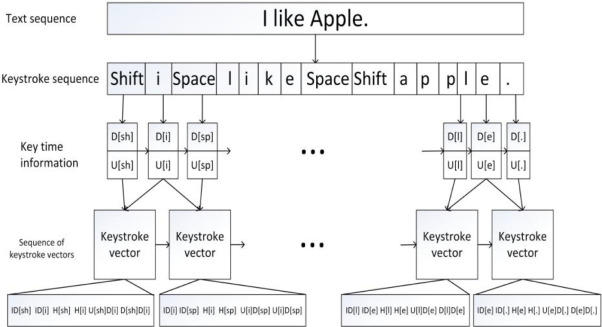
\includegraphics[width=0.5\textwidth]{images/vectorization.jpg}
	\caption{Vector data format transform by the authors of \cite{deep_learning}}
	\label{fig:deep_learning_vector_data_format}
\end{figure}

Then, the authors proposed multiple configurations of the neural network architecture. However, the more effecive can be see in the image \ref{fig:deep_learning_architecture}.

\begin{figure}[H]
	\centering
	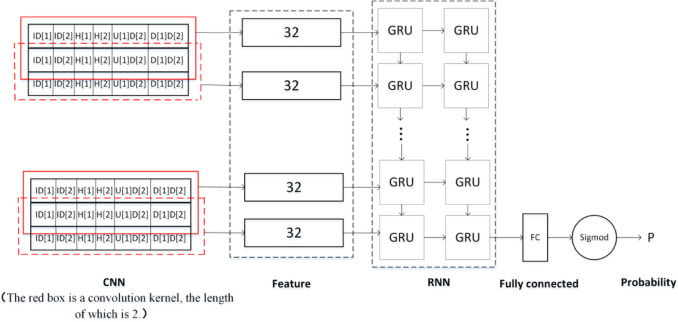
\includegraphics[width=0.5\textwidth]{images/architecture.jpg}
	\caption{Neural network architecture proposed by the authors of \cite{deep_learning}}
	\label{fig:deep_learning_architecture}
\end{figure}

As it can be seen, all the vectors extracted from a given text with specifict lenght in terms of keystrokes are arrange as a matrix where each row is a vector. Then, a one dimensional CNN with a convolutional kernel with lenght 2 (feature vectors) is applied to the matrix to extract 32 the features that are going to be used by the RNN, a double layer GRU. Finally, the output of the RNN connected to the fully-connected layer and then to the output layer, which is a sigmoid function that outputs the probability of the user being the user that the model is trying to identify. The authors also added droutout layers to each layer of the model to avoid overfitting.

This approach obtained a FRR of 2.07\%, a FAR of 3.26\% and an EER of 2.67\% using the Clarkson II dataset and a FRR of 6.61\%, a FAR of 5.31\% and an EER of 5.97\% using the Buffalo dataset.